\documentclass{beamer}


% ---
% PACOTES
% ---

% ---
% Pacotes fundamentais 
% ---
\usepackage{times}         % Usa a fonte Latin Modern
\usepackage[T1]{fontenc}      % Selecao de codigos de fonte.
\usepackage[utf8]{inputenc}      % Codificacao do documento (conversão automática dos acentos)
\usepackage{indentfirst}      % Indenta o primeiro parágrafo de cada seção.
\usepackage{nomencl}          % Lista de simbolos
\usepackage{color}            % Controle das cores
\usepackage{graphicx}         % Inclusão de gráficos
\usepackage{microtype}        % para melhorias de justificação
% ---
% ---
% Pacotes adicionais, usados apenas no âmbito do Modelo Canônico do abnteX2
% ---
\usepackage{lipsum}           % para geração de dummy text
% ---
      
% ---
% Pacotes de citações
% ---
\usepackage[brazilian,hyperpageref]{backref}  % Paginas com as citações na bibl
\usepackage[alf]{abntex2cite} % Citações padrão ABNT
% ---

% ---
% Configurações do pacote backref
% Usado sem a opção hyperpageref de backref
\renewcommand{\backrefpagesname}{Citado na(s) página(s):~}
% Texto padrão antes do número das páginas
\renewcommand{\backref}{}
% Define os textos da citação
\renewcommand*{\backrefalt}[4]{
   \ifcase #1 %
      Nenhuma citação no texto.%
   \or
      Citado na página #2.%
   \else
      Citado #1 vezes nas páginas #2.%
   \fi}%
% ---
\usetheme{Berlin}

% --- Informações de dados para CAPA e FOLHA DE ROSTO ---
\title{Atividade Energia - Planejamento de uma política pública}

\author{João Henrique da Silva -\
Maria Angélica Germani -\
Kassia Nascimento -\
Jonathan Santos Pericinoto}

\institute{UEM DCI PROFCIAMB}
\logo{

\includegraphics[width=1cm]{logo.png}

\includegraphics[width=1cm]{uem.png}
}

%\local{Brasil}
\date{Junho - 2022}
% ---

% ---
% Configurações de aparência do PDF final

% alterando o aspecto da cor azul
\definecolor{blue}{RGB}{41,5,195}

% informações do PDF
\makeatletter
\hypersetup{
      %pagebackref=true,
      pdftitle={\@title}, 
      pdfauthor={\@author},
      pdfsubject={},
      pdfcreator={},
      pdfkeywords={abnt}{latex}{abntex}{abntex2}{atigo científico}, 
      colorlinks=true,           % false: boxed links; true: colored links
      linkcolor=blue,            % color of internal links
      citecolor=blue,            % color of links to bibliography
      filecolor=magenta,            % color of file links
      urlcolor=blue,
      bookmarksdepth=4
}
\makeatother
% --- 

% ---
% compila o indice
% ---
\makeindex
% ---



% --- 
% Espaçamentos entre linhas e parágrafos 
% --- 

% O tamanho do parágrafo é dado por:
\setlength{\parindent}{1.3cm}

% Controle do espaçamento entre um parágrafo e outro:
\setlength{\parskip}{0.2cm}  % tente também \onelineskip

% Espaçamento simples
\linespread{1.3}


%\usetheme{lucid}
\begin{document}
    \frame {
        \titlepage
    }
    \frame {
        \frametitle{Escopo espacial do atendimento}
        \framesubtitle{Fatores históricos}
	\begin{itemize}
		\item Programa luz no campo; 2002 atendeu 90,8 por cento da população em regiões ermas, levando eletricidade 
		\item Custo 1996 - 1998 1,77 bilhões; subsídios
		\item Foco nas tecnologias de distribuição; direcionamento estatal das atividades no mercado de energia
	\end{itemize}
    }

    \frame{
        \frametitle{Stakeholders}
        \framesubtitle{}
        \begin{itemize}
            \item Ministério de minas e energia
            \item Operador nacional do sistema - Distribuição de energia
            \item Eletrobrás, Smart Grid - Rede Inteligente \cite{Energy_Storage_Smart_Grids}
        \end{itemize}
    }

    \frame{
        \frametitle{Público atendido}
        \framesubtitle{Políticas públicas}
        \begin{itemize}
            \item Urbanização; Industrialização; Consumo doméstico
            \item Fatores previstos em \cite{Potencial_Energeticos_2050}
            \item Imperativo do desenvolvimento sustentável \cite{Agenda_2030}
        \end{itemize}
    }

    \frame{
        \frametitle{Reservas energéticas}
        \framesubtitle{Fatores conjunturais - Petróleo}
        \begin{itemize}
            \item Petróleo - Reservas provadas aumentaram de 15 para 27 anos; autossuficiência; Pré-sal.
            \item 2,6 milhões de barris/dia em 2016 e subindo
            \item Brasil, um dos maiores produtores do mundo
        \end{itemize}
    }

    \frame{
        \frametitle{Reservas energéticas}
        \framesubtitle{Fatores conjunturais - Gás natural}
        \begin{itemize}
            \item Gás natural campos Marítimos e terrestres
            \item Previsão para 2050 - 200 milhões de metros cúbicos - Marítimo
            \item Previsão para 2050 - 450 milhões de metros cúbicos - Marítimo + terrestre
        \end{itemize}
    }

    \frame{
        \frametitle{Reservas energéticas}
        \framesubtitle{Fatores conjunturais - Urânio}
        \begin{itemize}
            \item Urânio Reservas exploradas 309 mil toneladas
            \item Urânio Reservas não exploradas 300 mil toneladas
            \item 187 mil toneladas de urânio recuperável, suficiente para 60 anos de funcionamento das Usinas Angra
            \item Domínio completo do ciclo de produção do combustível nuclear; da mineração ao enriquecimento
        \end{itemize}
    }

    \frame{
        \frametitle{Reservas energéticas}
        \framesubtitle{Fatores conjunturais - Carvão Mineral}
        \begin{itemize}
            \item Pouca expressão; 9,7 milhões de ton; capacidade instalada 3,2 GW
            \item Reservas poderiam garantir até 46 usinas de 500 MW durante 25 anos
            \item carece de investimentos em pesquisa exploração
            \item Altamente poluente e espalha radiação pelo ambiente \cite{radiological_coal-fired}
        \end{itemize}
    }

    \frame{
        \frametitle{Reservas energéticas}
        \framesubtitle{Fatores conjunturais - Biomassa}
        \begin{itemize}
            \item Diversas fontes de biomassa cana-de-açúcar, óleos e gorduras, resíduos rurais e urbanos
            \item Planejamento da EPE prevê que a expansão desta forma de energia não trará desmatamento e trará ganhos de produtividade para outras atividades correlatas
            \item Espera-se que em 2050 a disponibilidade seja equivalente à 530 milhões de toneladas de petróleo 
        \end{itemize}
    }

    \frame{
        \frametitle{Reservas energéticas}
        \framesubtitle{Fatores conjunturais - Hidrelétrica}
        \begin{itemize}
            \item Potencia de 176 GW; dos quais 108 Gw já aproveitados
            \item Custos de implantação e impacto socioambiental alto
            \item Hidrografia da Amazônia, Tocantis-Araguaia protegida por territórios indígenas
            \item PCH - Pequenas centrais hidrelétricas;  modelo alternativo que pode ser anexado à outras infraestruturas de transporte fluviais e canais.
        \end{itemize}
    }

    \frame{
        \frametitle{Reservas energéticas}
        \framesubtitle{Fatores conjunturais - Eólica (onshore \& offshore)}
        \begin{itemize}
            \item Enorme potencial 143 GW onshore - 50m; em alturas superiores até 440 GW
            \item Offshore distante até 10km 57GW; dentro da ZEE - 200km, 1780 GW
            \item Offshore profundidade até 0-20m - 176 GW
            \item Offshore profundidade até 20-50m - 223 GW
            \item Offshore profundidade até 50-100m - 606 GW
        \end{itemize}
    }

    \frame{
        \frametitle{Reservas energéticas}
        \framesubtitle{Fatores conjunturais - Eólica Solar (onshore \& offshore)}
        \begin{itemize}
            \item Enorme potencial 506 TWh/ano
            \item Fotovoltaica residencial distribuída 287 TWh/ano
            \item Offshore 94706 TWh/ano
            \item Energia Heliotérmica cilindro parabólico 661 TWh/ano
            \item Energia Heliotérmica torre solar 359 TWh/ano
        \end{itemize}
    }

    \frame{
        \frametitle{Reservas energéticas}
        \framesubtitle{Fatores conjunturais - Oceânica e outra fontes}
        \begin{itemize}
            \item Pouco desenvolvida, necessita de investimentos; 114 Gw
            \item Reservas de metano, nitrogênio, hélio, hidrogênio natural e outros gases extraídos de poços são uma mercadoria valorizada
        \end{itemize}
    }

    \frame{
        \frametitle{Expansão da produção de Energia PDE 2030}
        \begin{figure}
          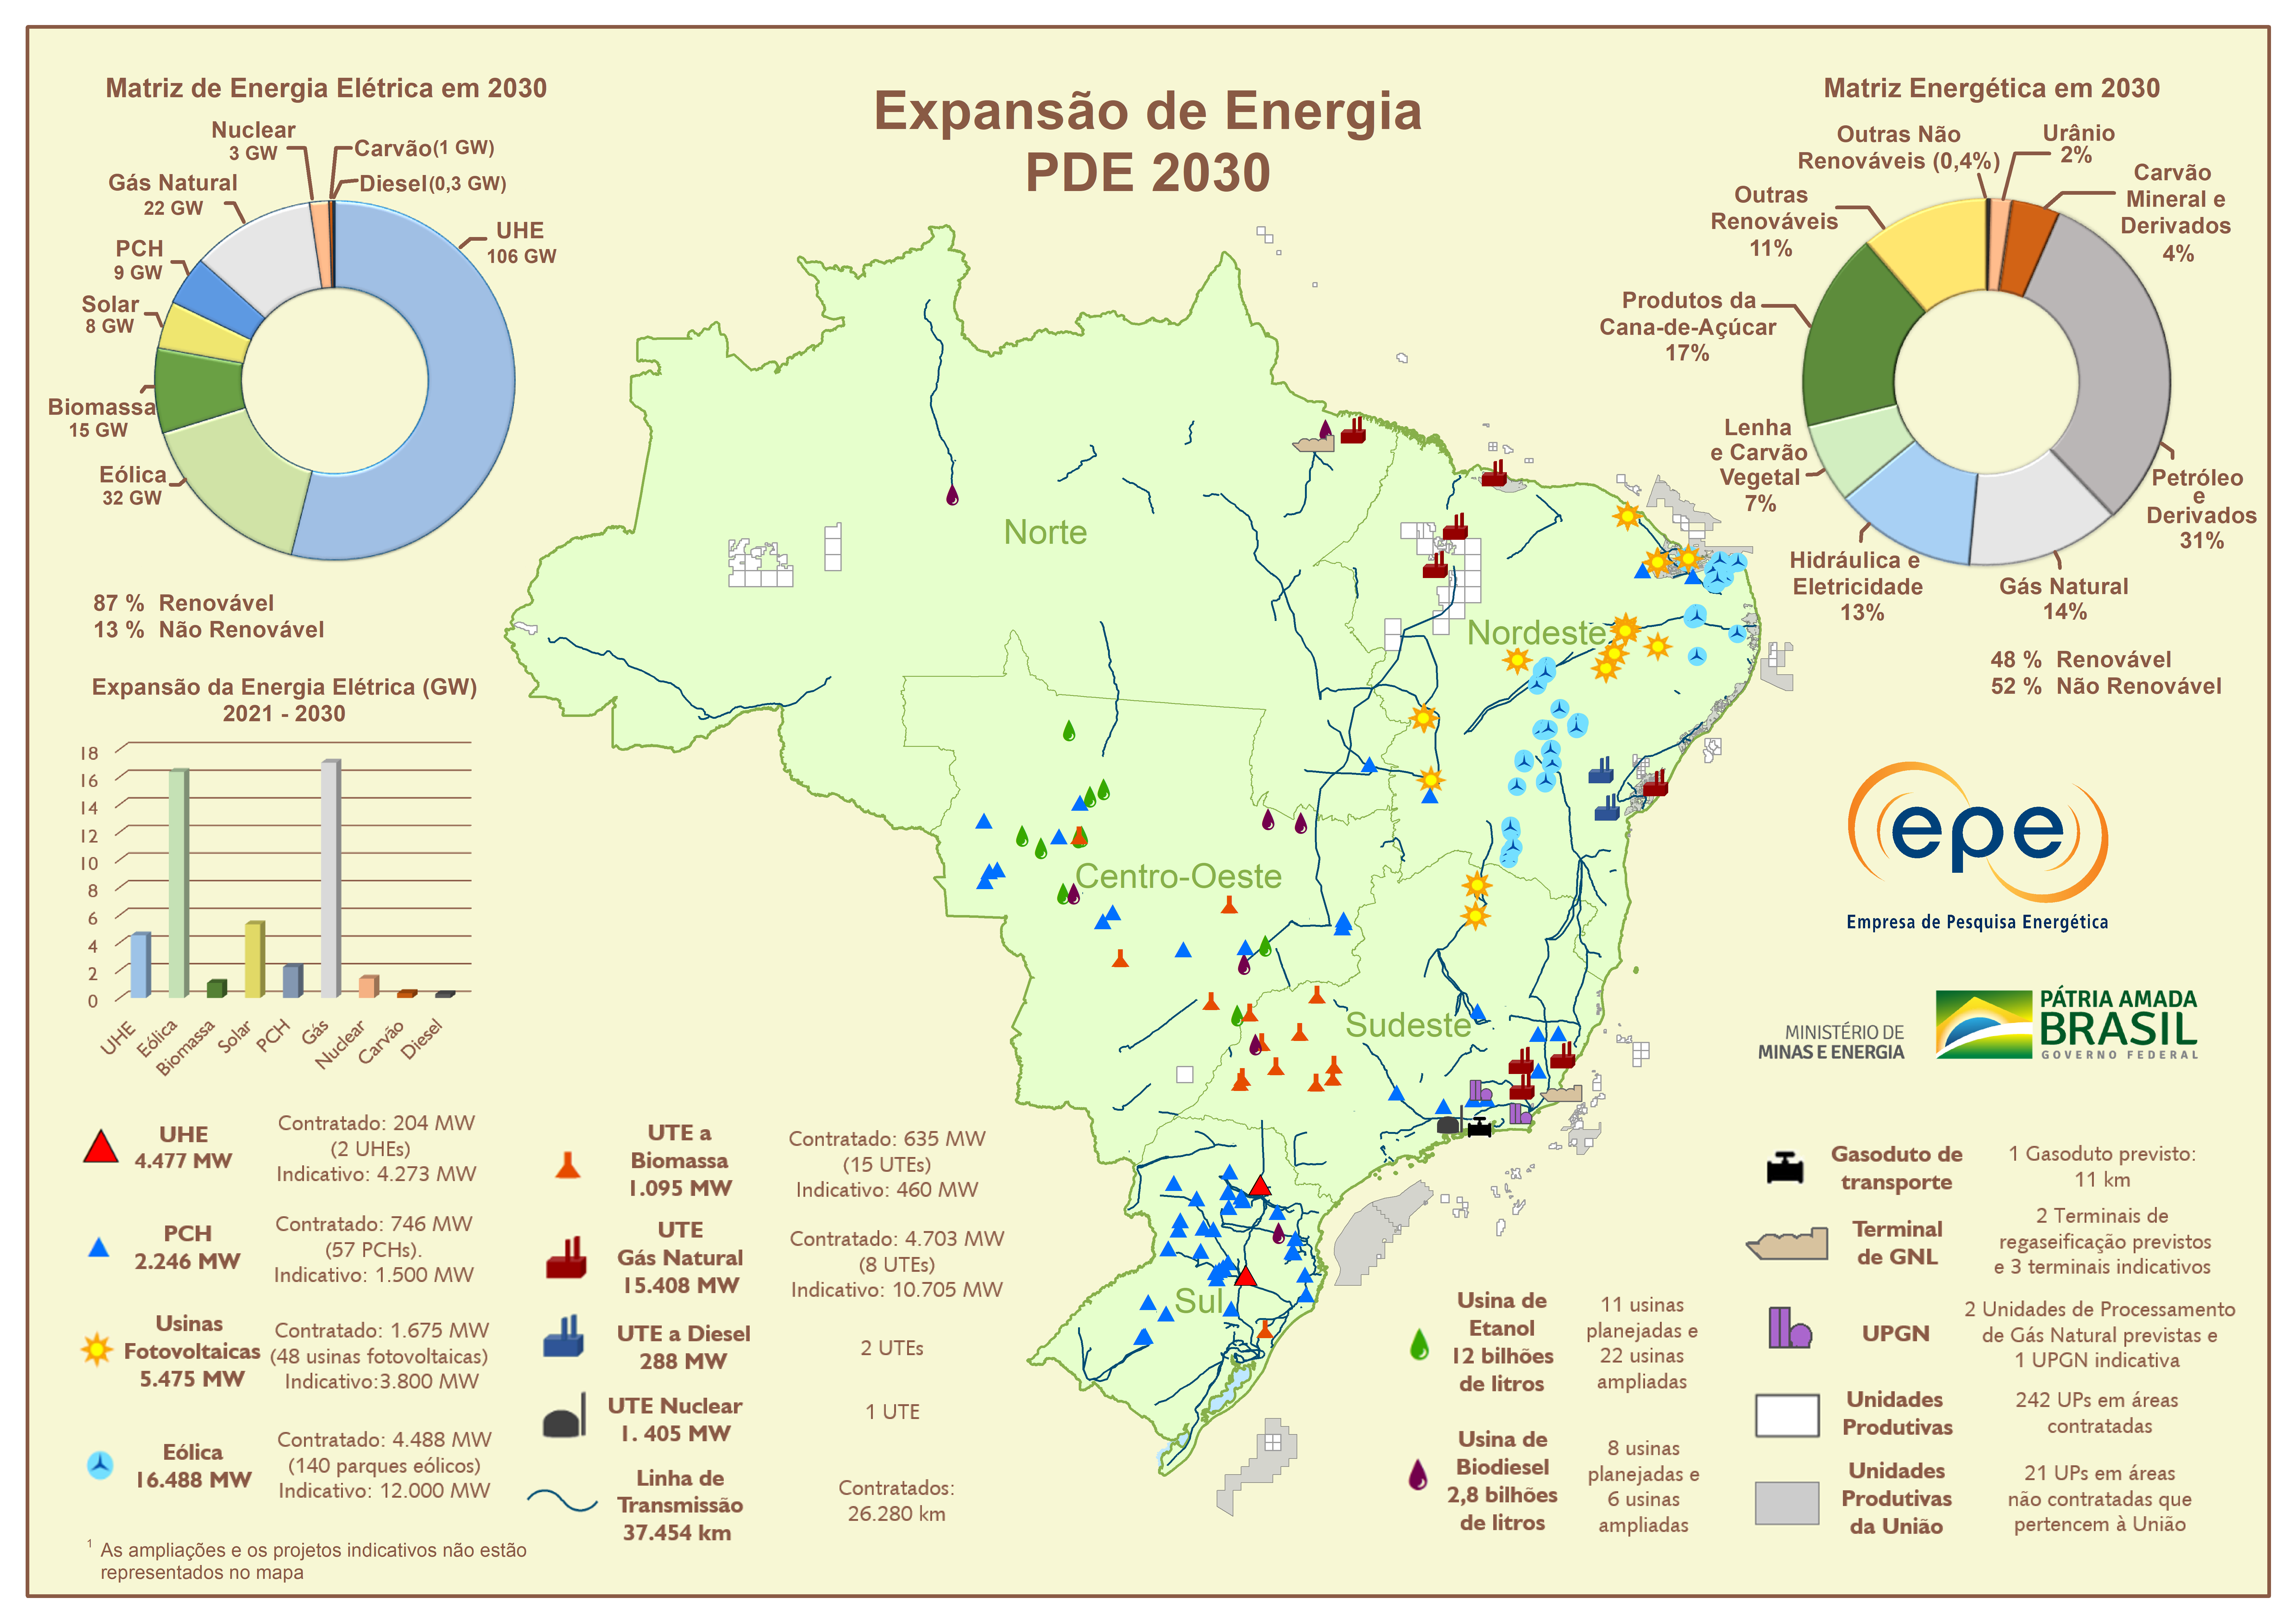
\includegraphics[scale=0.18]{A3_Expansao_Energia_PDE2030_02_21.png}
        \end{figure}
    }


    \frame{
        \frametitle{Dimensionamento das necessidades}
        \framesubtitle{Geração prevista pros próximos anos \cite[p.29]{Plano_Expansao_Energia_2030}}
        \begin{figure}
          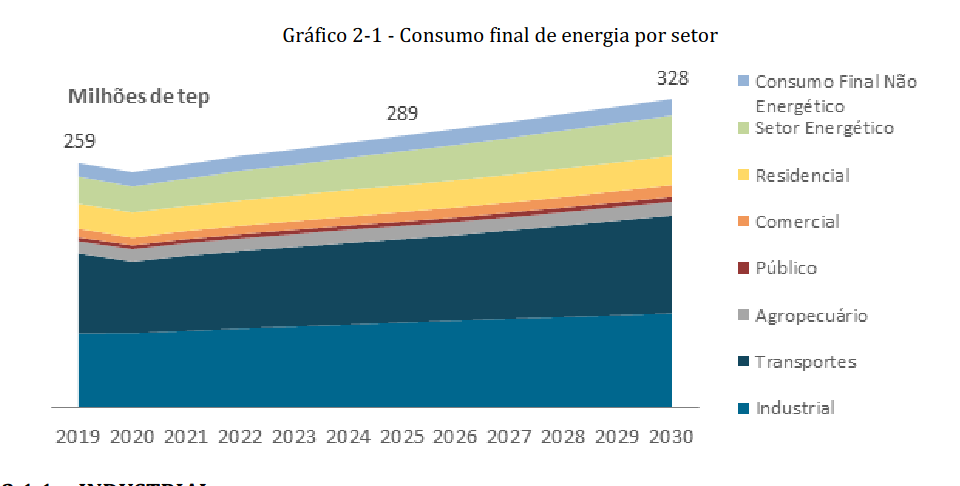
\includegraphics[scale=0.4]{consumo_final.png}
        \end{figure}
    }

    \frame{
        \frametitle{Impacto ambiental das alternativas - 1}
        \begin{table}
        \centering
        \caption{Formas de geração de energia e impacto ambiental \cite{Climate_quantitative_projections}}
        \begin{tabular}{lll}
                      & Renovável & Limpa  \\
        Hidroelétrica & Sim       & Sim    \\
        Termoelétrica & Não       & Não    \\
        Termonuclear  & Não       & Sim    \\
        Eólico        & Sim       & Sim    \\
        Fotovoltaica  & Sim       & Sim    \\
        Biomassa      & Sim       & Não   
        \end{tabular}
        \end{table}
    }

    \frame{
        \frametitle{Impacto ambiental das alternativas - 2}
        \begin{table}
        \centering
        \caption{Proporção das formas de geração de energia}
        \begin{tabular}{llll}
                          & Total produzido & Proporção 1  & Proporção 2  \\
        Itaipú            & 14000 MW        & 1            & 1            \\
        336 Aerogeradores & 8195 MW         & 1.70835      & 0.58535      \\
        1 Aerogerador     & 25 MW           & 560          & 0.00178      \\
        Angra 1           & 640 MW          & 21.875       & 0.04571      \\
        Angra 2           & 1350 MW         & 10.370       & 0.09642      \\
                          &                 &              &              \\
                          &                 &              &             
        \end{tabular}
        \end{table}
    }

\newpage

\bibliography{Interdisciplinaridade}

\end{document}


